% !TeX program = pdfLaTeX
\documentclass[smallextended]{svjour3}       % onecolumn (second format)
%\documentclass[twocolumn]{svjour3}          % twocolumn
%
\smartqed  % flush right qed marks, e.g. at end of proof
%
\usepackage{amsmath}
\usepackage{graphicx}
\usepackage[utf8]{inputenc}

\usepackage[hyphens]{url} % not crucial - just used below for the URL
\usepackage{hyperref}

%
% \usepackage{mathptmx}      % use Times fonts if available on your TeX system
%
% insert here the call for the packages your document requires
%\usepackage{latexsym}
% etc.
%
% please place your own definitions here and don't use \def but
% \newcommand{}{}
%
% Insert the name of "your journal" with
% \journalname{myjournal}
%

%% load any required packages here



% tightlist command for lists without linebreak
\providecommand{\tightlist}{%
  \setlength{\itemsep}{0pt}\setlength{\parskip}{0pt}}

% From pandoc table feature
\usepackage{longtable,booktabs,array}
\usepackage{calc} % for calculating minipage widths
% Correct order of tables after \paragraph or \subparagraph
\usepackage{etoolbox}
\makeatletter
\patchcmd\longtable{\par}{\if@noskipsec\mbox{}\fi\par}{}{}
\makeatother
% Allow footnotes in longtable head/foot
\IfFileExists{footnotehyper.sty}{\usepackage{footnotehyper}}{\usepackage{footnote}}
\makesavenoteenv{longtable}

% Pandoc citation processing
\newlength{\cslhangindent}
\setlength{\cslhangindent}{1.5em}
\newlength{\csllabelwidth}
\setlength{\csllabelwidth}{3em}
\newlength{\cslentryspacingunit} % times entry-spacing
\setlength{\cslentryspacingunit}{\parskip}
% for Pandoc 2.8 to 2.10.1
\newenvironment{cslreferences}%
  {}%
  {\par}
% For Pandoc 2.11+
\newenvironment{CSLReferences}[2] % #1 hanging-ident, #2 entry spacing
 {% don't indent paragraphs
  \setlength{\parindent}{0pt}
  % turn on hanging indent if param 1 is 1
  \ifodd #1
  \let\oldpar\par
  \def\par{\hangindent=\cslhangindent\oldpar}
  \fi
  % set entry spacing
  \setlength{\parskip}{#2\cslentryspacingunit}
 }%
 {}
\usepackage{calc}
\newcommand{\CSLBlock}[1]{#1\hfill\break}
\newcommand{\CSLLeftMargin}[1]{\parbox[t]{\csllabelwidth}{#1}}
\newcommand{\CSLRightInline}[1]{\parbox[t]{\linewidth - \csllabelwidth}{#1}\break}
\newcommand{\CSLIndent}[1]{\hspace{\cslhangindent}#1}

% Jese tex
\hypersetup{hidelinks}
\usepackage[hyphenbreaks]{breakurl}
\usepackage[hyphens]{url}


\usepackage{booktabs}
\usepackage{longtable}
\usepackage{array}
\usepackage{multirow}
\usepackage{wrapfig}
\usepackage{float}
\usepackage{colortbl}
\usepackage{pdflscape}
\usepackage{tabu}
\usepackage{threeparttable}
\usepackage{threeparttablex}
\usepackage[normalem]{ulem}
\usepackage{makecell}
\usepackage{xcolor}
\begin{document}


\title{Achieving Analytical Fluency With Complex Data \thanks{The authors acknowledge EPSRC grant: EP/R513088/1 for funding the doctoral research on which this work is based.} }
 \subtitle{Refining the analytical process} 

    \titlerunning{Analytical Fluency}

\author{  Paul J Palmer \and  Michael Henshaw \and  Russell Lock \and  }

    \authorrunning{ P.J. Palmer, M. Henshaw, R.L. Lock }

\institute{
        Paul J Palmer \at
     Department of YYY, University of XXX \\
     \email{\href{mailto:abc@def}{\nolinkurl{abc@def}}}  %  \\
%             \emph{Present address:} of F. Author  %  if needed
    \and
        Michael Henshaw \at
     Department of ZZZ, University of WWW \\
     \email{\href{mailto:djf@wef}{\nolinkurl{djf@wef}}}  %  \\
%             \emph{Present address:} of F. Author  %  if needed
    \and
        Russell Lock \at
     Department of ZZZ, University of WWW \\
     \email{\href{mailto:djf@wef}{\nolinkurl{djf@wef}}}  %  \\
%             \emph{Present address:} of F. Author  %  if needed
    \and
    }

\date{Received: date / Accepted: date}
% The correct dates will be entered by the editor


\maketitle

\begin{abstract}
Scientific analysis is formally presented as a rigid process typically
Experiment; Analysis, Evaluation; and Conclusions.
comprising: Review; Theory; Research question; Methodology;
We do, however, question whether established methods for managing and
analysing data are still appropriate for ``Big Data'', by which we mean
data that is too big to be conveniently manipulated by manually
intensive methods.
is to justify why there is a need for new analytical techniques, given
that the existing ones still work; the second is to show how an
abstract perception of data impacts the analytical process.
This presents two questions which we seek to address here: the first
An example of the motivation for change is illustrated by the ``Grammar
of Graphics'' (GoG) paradigm. GoG uses combinations of transforms to
generate every possible graphic and tabulation from data presented in
a suitable state allowing for a radical change in the analytic
workflow, while still preserving the goals of scientific analysis.
By framing this problem as one of transforming \emph{data state}, we can
mathematically describe general properties allowing the creation of
re-usable code templates for data preparation. Coupled with ``literate
programming'' techniques we show that this approach enables
analytically fluent analysis of complex data.
\\
\keywords{
        key \and
        dictionary \and
        word \and
    }


\end{abstract}


\def\spacingset#1{\renewcommand{\baselinestretch}%
{#1}\small\normalsize} \spacingset{1}


\hypertarget{sec:introduction}{%
\section{Introduction}\label{sec:introduction}}

Scientific analysis is formally presented as a rigid process typically comprising: Review; Theory; Research question; Methodology; Experiment; Analysis, Evaluation; and Conclusions. This is a powerful framework that has stood the test of time which is the underlying format of countless academic publications. But just because this format is rigid, does not mean that there is no opportunity to improve the method used to achieve it.

If we look deeper, we can start to separate the actual process of scientific discovery from the way in which it is reported. The documentation of research and analysis that has already been completed, is very different to an exploration where the outcomes are as yet unknown. Nobel Prize winner Szent-Györgyi (1972) discussed this issue in 1972, long before the age of computers and ``Big Data''\footnote{By ``Big Data'' we mean data that is too big to be conveniently manipulated by manually intensive methods.} introduced computational and data intensive research methods~(Szent-Györgyi 1972). He described the Apollonian as following a formally prescribed research path while a Dionysian explores the unknown. However, research and reporting are necessarily linked and one should be a clear and true interpretation of the other.

We argue here that this presumption the analytical process should follow the final method of presentation is a hindrance to the adoption of new analytical techniques. The term ``reproducible research'' has been coined to describe this linkage, without defining how it may be achieved, leading to discussion on the topic by~(Stodden, Leisch, and Peng 2014; Lewis, Vander Wal, and Fifield 2018; Leeper 2014; Gentleman and Temple Lang 2007; Peng 2015; Drummond 2018) and others.

Two questions arise from these discussions which we seek to address in the following sections: the first is to justify why there is a need for new analytical techniques, given that the existing ones still work? The second relates to the concepts we introduce in this work: how can changing our abstract perception of data beneficially impact the analytical process?

Both the need and benefit are illustrated by the ``Grammar of Graphics'' (GoG) paradigm (Wilkinson 2010). GoG uses combinations of transforms to generate every possible graphic and tabulation from data that is presented in a suitable state. Thus, a researcher planning to use GoG will focus on saving research data in suitable state, so she can make many dynamic visualisations as work progresses, rather than waiting for the end of the data collation phase.

This contrasts with the typical approach where difficulties with data intensive analysis are often retrospectively blamed on imperfections within the data that are seen as requiring ``cleaning'' before analysis can begin. It is unfortunate that the popular spreadsheet encourages a manually intensive formatting of data and the use of visualisation tools that do not scale well with data size (Mack et al. 2018; Bishop 2013; Powell, Baker, and Lawson 2008).

Our alternative approach is consider data as observations of the real world that are to be interpreted through analysis, rather than formatted tables meeting arbitrary technical specifications. This also expands on an idea hinted at in the GoG example above: there is no need to rigidly define data format in advance since the real world is clearly independent of the methods we choose to observe and record. If we believe that the knowledge we seek is encapsulated within a set of observations, then we can choose a viewpoint where we see data as starting in an initial \emph{inconvenient state}. It follows that we must transform it into a \emph{convenient state} for analysis. By constructing a working theory supported with a mathematical description, we show that the transformation of \emph{data state} can be generalised to allow the creation of re-usable code templates. To explain how re-framing the problem of \emph{imperfect data} in terms of \emph{data state} can make such a difference to the way in which we approach the analytical process, we must first construct a methodology that takes into account the nature of data.

\hypertarget{sec:methodology}{%
\section{Methodology}\label{sec:methodology}}

The two questions we seek to answer are: ``Why develop new analytical techniques, given that the existing ones still work?'' and ``How can changing our abstract perception of data beneficially impact the analytical process?'' To achieve this goal we follow a pragmatic methodology that draws inspiration from the critical realism philosophy of (Bhaskar 2008) which gives context to data as observations arising from an unknowable real world. Our methodology is pragmatic in that we use public domain weather data as the case study for each step in our analytical approach. This data has the following characteristics:

\begin{itemize}
\tightlist
\item
  Open Source;
\item
  Presented in an inconvenient state for analysis;
\item
  Multiple units of measure;
\item
  Extensible, in that related similar sources are available.
\end{itemize}

We do not, however, try to justify the analytical \emph{results} from our case study, as the intent of this work is to demonstrate how \emph{analytical fluency} can be achieved when faced with the complexities of real data. The reason for this caveat is due the topical subject of the case study and how it relates to the future of the real world. We emphasise that our analysis of past events is not a model for extrapolating future events.

In early drafts of this work, the case study was envisaged as a separate document, but this approach felt very artificial, and the benefits of fluency were unconvincing when presented in this way. We have rewritten it so in a recursive sense this article is a case study about the techniques used to write it. This presents a challenge on how best to structure this document to convey the essentials of the techniques we propose and allow the reader to critique the approach.

A further challenge is that that the final output will be a static document rendered from the dynamic components and will look no different from any other document. Since we cannot produce a dynamic document on paper, we will produce a report and a presentation from the same data using the same reusable elements. Given that the weather data is regularly updated though time, and there are many sources of such data, we aim to show that the overall effort of creating documents using analytically fluent methodologies is much less than repeating the same work with manually intensive processes.

The work is presented in the following order:

\begin{itemize}
\tightlist
\item
  Data Definition:

  \begin{itemize}
  \tightlist
  \item
    Consider the philosophical nature of data with special reference to the case study to create a data model.
  \end{itemize}
\item
  Apply the model:

  \begin{itemize}
  \tightlist
  \item
    The practical demonstration of data ready for analysis.
  \end{itemize}
\item
  Template Concept:

  \begin{itemize}
  \tightlist
  \item
    Building reusable programmatic elements for analysis.
  \end{itemize}
\item
  Template Evaluation:

  \begin{itemize}
  \tightlist
  \item
    A demonstration and evaluation of the template and its role in supporting analytical fluency.
  \end{itemize}
\end{itemize}

Throughout this work we have based the practical analysis on the R Analytical language (R Core Team 2022). In principle, the techniques presented here would work with other languages such as Python (Gentleman and Temple Lang 2007), but their potential has not been explored. The detailed implementation can be found at the Github repository xxxxxxx. A presentation using the same code elements is also presented alongside the ``paper'' format. While this serves to demonstrate the re-usability of code, it was created as a container for the visualisations used prior to the creation of the supporting narrative. Simply put, it was easier to create both presentation and report.

\hypertarget{sec:case-study}{%
\section{Case Study Data}\label{sec:case-study}}

\begin{figure}

{\centering 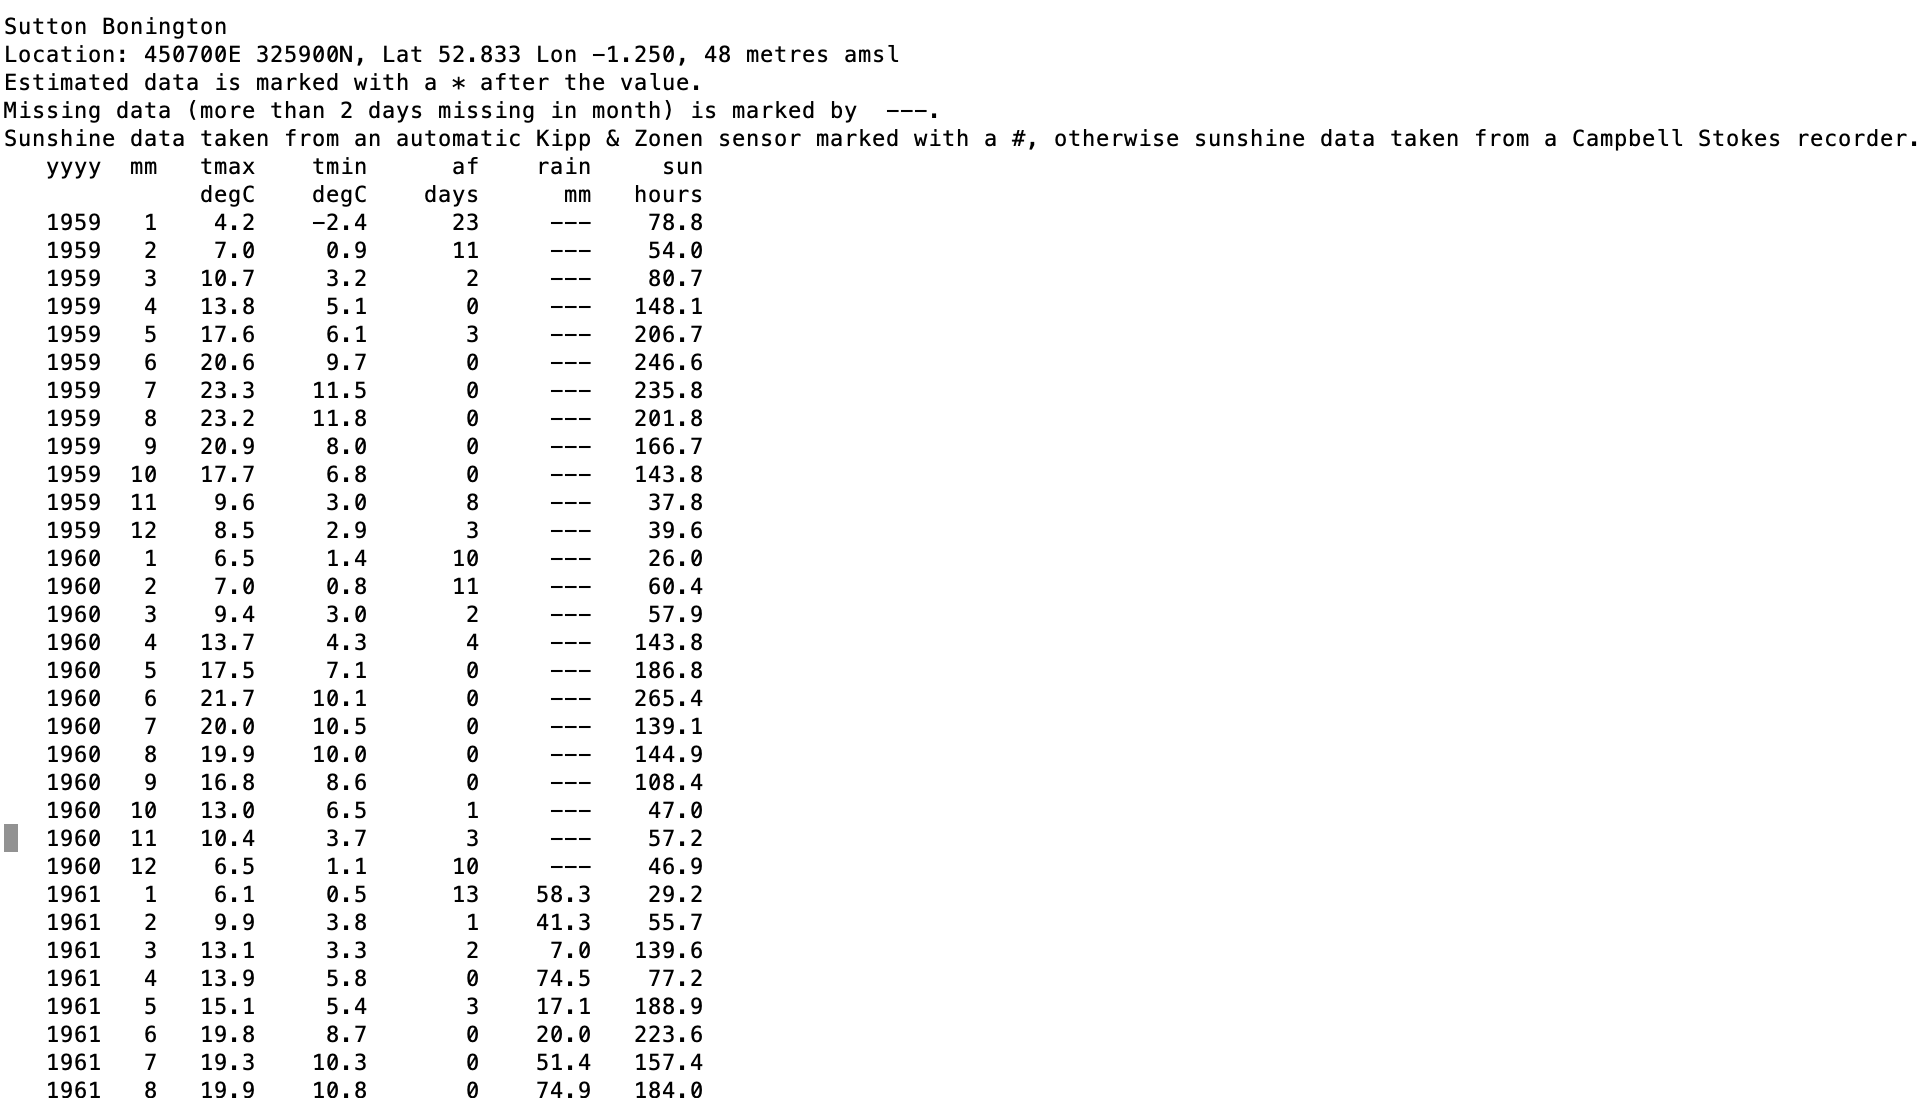
\includegraphics[width=0.7\linewidth]{image_Sutton_bonnington_data} 

}

\caption{Source data showing the initial inconvenient state for analysis.}\label{fig:ImageSuttonBonningtonData}
\end{figure}

The case study uses data from the Sutton Bonnington long term weather monitoring station which is freely available online from (UK Metrological Office 2022). As Figure \ref{fig:ImageSuttonBonningtonData} shows, it contains observations from 1959 to the present day, and is presented as a text file in an inconvenient format for analysis. The files contain a series of weather related observations in various units. To complicate matters some are annotated and some are missing.

However, if we unpick the file shown in Figure \ref{fig:ImageSuttonBonningtonData} we can see that the UK Metrological Office statement that the file contains a ``time series of monthly data'' is true, but the data is not useable ``as is'' due to the way in which it is formatted. If we were to alter the observations it contains into a series of columns labelled: Date, Maximum temperature, Minimum temperature, etc., we would accept these as data for analysis, and possibly even present this revised format as ``raw data'' in a formal report with the justification that ``nothing has been changed.''

Our reason for emphasising these points are to lay the foundation for
introducing a terminology of ``data state'' to describe the changes in
data presentation that do not affect the inherent knowledge contained
within it. Looking ahead to Table 1 and our terminology it is clear that the data as supplied is what we term as Data \emph{nascent} and that the \emph{Nominal} data fields are equivalent to the column format proposed earlier in the previous paragraph. These interpretations are based entirely on what we believe the data represents about the real world and our analytical intent, if our research was to examine the observational impact of changes in meteorological recording equipment in the accuracy of long term records, then we would clearly need additional nominal data fields.

\hypertarget{references}{%
\section*{References}\label{references}}
\addcontentsline{toc}{section}{References}

\hypertarget{refs}{}
\begin{CSLReferences}{1}{0}
\leavevmode\vadjust pre{\hypertarget{ref-Bhaskar2008}{}}%
Bhaskar, Prof. Roy. 2008. \emph{{A Realist Theory of Science}}. London, UK: Verso.

\leavevmode\vadjust pre{\hypertarget{ref-Bishop2013}{}}%
Bishop, Katrina. 2013. {``{Spreadsheet blunders costing business billions}.''} Englewood Cliffs, New Jersey,USA. \url{https://www.cnbc.com/id/100923538}.

\leavevmode\vadjust pre{\hypertarget{ref-Drummond2018}{}}%
Drummond, Chris. 2018. {``{Reproducible research: a minority opinion}.''} \emph{Journal of Experimental and Theoretical Artificial Intelligence} 30 (1): 1--11. \url{https://doi.org/10.1080/0952813X.2017.1413140}.

\leavevmode\vadjust pre{\hypertarget{ref-Gentleman2007}{}}%
Gentleman, Robert, and Duncan Temple Lang. 2007. {``{Statistical Analyses and Reproducible Research}.''} \emph{Journal of Computational and Graphical Statistics} 16 (1): 1--23. \url{https://doi.org/10.1198/106186007X178663}.

\leavevmode\vadjust pre{\hypertarget{ref-Leeper2014}{}}%
Leeper, J., Thomas. 2014. {``{Archiving Reproducible Research with R and Dataverse}.''} \emph{The R Journal} 6 (1): 151. \url{https://doi.org/10.32614/RJ-2014-015}.

\leavevmode\vadjust pre{\hypertarget{ref-Lewis2018a}{}}%
Lewis, Keith P., Eric Vander Wal, and David A. Fifield. 2018. {``{Wildlife biology, big data, and reproducible research}.''} \emph{Wildlife Society Bulletin} 42 (1): 172--79. \url{https://doi.org/10.1002/wsb.847}.

\leavevmode\vadjust pre{\hypertarget{ref-Mack2018}{}}%
Mack, Kelly, John Lee, Kevin Chang, Karrie Karahalios, and Aditya Parameswaran. 2018. {``{Characterizing Scalability Issues in Spreadsheet Software using Online Forums}.''} University of Illinois. \url{http://arxiv.org/abs/1801.03829}.

\leavevmode\vadjust pre{\hypertarget{ref-Peng2015}{}}%
Peng, Roger. 2015. {``{The reproducibility crisis in science: A statistical counterattack}.''} \emph{Significance} 12 (3): 30--32. \url{https://doi.org/10.1111/j.1740-9713.2015.00827.x}.

\leavevmode\vadjust pre{\hypertarget{ref-Powell2008}{}}%
Powell, Stephen G., Kenneth R. Baker, and Barry Lawson. 2008. {``{A critical review of the literature on spreadsheet errors}.''} \emph{Decision Support Systems} 46 (1): 128--38. \url{https://doi.org/10.1016/j.dss.2008.06.001}.

\leavevmode\vadjust pre{\hypertarget{ref-RCoreTeam2017}{}}%
R Core Team. 2022. {``{R: A language and environment for statistical computing. R Foundation for Statistical Computing}.''} Vienna, Austria: R Foundation for Statistical Computing. \url{https://www.r-project.org/}.

\leavevmode\vadjust pre{\hypertarget{ref-Stodden2014}{}}%
Stodden, Victoria, Friedrich Leisch, and Roger D. Peng. 2014. \emph{{Implementing reproducible research}}. CRC Press/Taylor; Francis.

\leavevmode\vadjust pre{\hypertarget{ref-Szent-Gyorgyi1972}{}}%
Szent-Györgyi, Albert. 1972. {``{Dionysians and apollonians}.''} \emph{Science} 176 (4038): 966. \url{https://doi.org/10.1126/science.176.4038.966}.

\leavevmode\vadjust pre{\hypertarget{ref-UKMetrologicalOffice2022}{}}%
UK Metrological Office. 2022. {``{UK Met Office Historic Station Data}.''}

\leavevmode\vadjust pre{\hypertarget{ref-Wilkinson2010}{}}%
Wilkinson, Leland. 2010. \emph{{The grammar of graphics}}. \url{https://doi.org/10.1002/wics.118}.

\end{CSLReferences}


\bibliographystyle{spphys}
\bibliography{library.bib}


\end{document}
